\section{Sturm-Liouville Theory}

\subsection{Review of second-order linear ODEs}
\textit{This section is a review of IA Differential Equations.}

We wish to solve a general inhomogeneous ODE, written
\begin{align} \label{eq:2.1}
    \mathcal L y \equiv \alpha(x) y'' + \beta(x) y' + \gamma(x) y = f(x)
\end{align}
The homogeneous version has $f(x) = 0$, so \begin{align} \label{eq:2.2}
    \mathcal{L}y = 0,
\end{align} which has two independent solutions $y_1, y_2$.
The general solution, also the complementary function for the inhomogeneous ODE, is 
\begin{align}
    y_c(x) = A y_1(x) + B y_2(x). \label{eq:2.3}
\end{align}

The inhomogeneous equation 
\begin{align}
    \mathcal L y = f(x) \label{eq:2.4}
\end{align} has a solution called the particular integral, denoted $y_p(x)$.
The general solution to this equation is then 
\begin{align} \label{eq:2.5}
    y(x) = y_p + y_c.
\end{align}

We need two boundary or initial conditions to find the particular solution to the differential equation.
Suppose $x \in [a,b]$.
We can create boundary conditions by defining $y(a), y(b)$, often called the Dirichlet conditions.
Alternatively, we can consider $y(a), y'(a)$, called the Neumann conditions.
We could also used some kind of mixed condition, for instance $y + ky'$.

Homogeneous boundary conditions are such that $y(a) = y(b) = 0$.
In this part of the course, homogeneous boundary conditions are often assumed.
Note that we can add a complementary function $y_c$ to the solution, for instance $\overline{y} = y + A y_1 + B y_2$ such that $\overline{y}(a) = \overline{y}(b) = 0$.
This would allow us to construct homogeneous boundary conditions even when they are not present \textit{a priori} in the problem.
We could also specify initial data, such as solving for $x \geq a$, given $y, y'$ at $x = a$.

To solve the inhomogeneous equation \cref{eq:2.1}, we want to use eigenfunction expansions (like FS \cref{eq:1.22}).
In order to do this, we must first solve the \underline{related} eigenvalue problem.
In this case, that is
\begin{align}
    \alpha(x) y'' + \beta(x) y' + \gamma(x) y = -\lambda \rho(x) y. \label{eq:2.6}
\end{align}
We must solve this equation with the same boundary conditions as the original problem.
This form of equation often arises as a result of applying a separation of variables, particularly for PDEs in several dimensions.

\subsection{Sturm-Liouville form}
\begin{definition}[Inner product]
    For two complex-valued functions $f, g$ on $[a,b]$, we define the inner product as
    \begin{align*}
        \inner{f,g} = \int_a^b f^\star(x) g(x) \dd{x}
    \end{align*} 
\end{definition} 
The eigenvalue problem \cref{eq:2.6} above greatly simplifies if $\mathcal L$ is \underline{self-adjoint}, that is, if it can be expressed in \underline{Sturm-Liouville form}:
\begin{align} \label{eq:2.7}
    \mathcal L y \equiv -(py')' + qy = \lambda w y.
\end{align}
$\lambda$ is an eigenvalue, and $w(x)$ is the \textit{weight function}, which must be non-negative $w(x) \geq 0 \ \forall \; x$.

\subsection{Converting to Sturm-Liouville form}
Multiply \cref{eq:2.6} by an integrating factor $F(x)$ to give
\begin{align*}
    F \alpha y'' + F \beta y' + F \gamma y &= -\lambda F \rho y \\
    \dv{x} \qty(F \alpha y') - F' \alpha y' - F \alpha' y' + F \beta y' + F \gamma y &= -\lambda F \rho y
\end{align*}
To eliminate the $y'$ term, we require $F'\alpha = F(\beta - \alpha')$.
Thus,
\begin{align}
    \frac{F'}{F} &= \frac{\beta - \alpha'}{\alpha} \notag \\
    \implies F &= \exp \int^x \frac{\beta - \alpha'}{\alpha} \dd{x} \label{eq:2.8}
\end{align}
and further,
\begin{align*}
    (F\alpha y')' + F \gamma y = - \lambda F \rho y
\end{align*}
hence
\begin{align*}
    p & = F \alpha \\
    q & = F \gamma \\
    w & = F \rho
\end{align*} in $\cref{eq:2.7}$ and $F(x) > 0$ hence $w > 0$.
\begin{example}
    Consider the Hermite equation for simple harmonic oscillator,
    \begin{align*}
        y'' - 2xy' + 2ny = 0
    \end{align*}
    In this case for \cref{eq:2.6} $\alpha = 1,\ \beta = -2x,\ \gamma = 0,\ \lambda p = 2n$.
    So by \cref{eq:2.8}
    \begin{align*}
        F = \exp \int^x \frac{-2x}{1} \dd{x} = e^{-x^2}
    \end{align*}
    Then the equation, in Sturm-Liouville form, is
    \begin{align}
        \mathcal L y \equiv -\qty(e^{-x^2} y')' = 2n e^{-x^2} y \label{eq:2.9}
    \end{align}
\end{example}

\subsection{Self-adjoint operators}
\begin{definition}[Self-adjoint operator]
    $\mathcal L$ is a self-adjoint operator on $[a,b]$ for all pairs of functions $y_1,y_2$ satisfying appropriate boundary conditions if
    \begin{align*}
        \inner{y_1, \mathcal L y_2} = \inner{\mathcal L y_1, y_2}
    \end{align*}
\end{definition}
Written explicitly,
\begin{align} \label{eq:2.10}
    \int_a^b y_1^\star(x) \mathcal L y_2(x) \dd{x} = \int_a^b (\mathcal L y_1(x))^\star y_2(x) \dd{x}
\end{align}

\underline{Boundary conditions}: Substituting Sturm-Liouville form \cref{eq:2.7} into the above,
\begin{align}
    \inner{y_1, \mathcal L y_2} - \inner{\mathcal L y_1, y_2} &= \int_a^b \qty[-y_1 (py_2')' + y_1 q y_2 + y_2 (p y_1')' - y_2 q y_1] \dd{x} \notag \\
    &= \int_a^b \qty[-y_1 (py_2')' + y_2 (p y_1')'] \dd{x} \notag
    \intertext{Adding $-y_1' p y_2' + y_1' p y_2'$,}
    &= \int_a^b \qty[-(py_1y_2')' + (py_1'y_2)'] \dd{x} \notag \\
    &= [-py_1y_2' + py_1'y_2]_a^b \label{eq:2.11}
\end{align}
which must be zero for an equation in Sturm-Liouville form to be self-adjoint.

\subsection{Self-adjoint compatible boundary conditions}
\begin{itemize}
    \item Suppose $y(a) = y(b) = 0$.
        Then certainly the Sturm-Liouville form of the differential equation is self-adjoint.
        We could also choose $y'(a) = y'(b) = 0$ or $y + ky' = 0$.
        Collectively, the act of using homogeneous boundary conditions is known as the \textit{regular} Sturm-Liouville problem.
    \item Periodic boundary conditions could also be used, such as $y(a) = y(b)$.
    \item If $a$ and $b$ are singular points of the equation, i.e.
        $p(a) = p(b) = 0$, this is self-adjoint compatible.
    \item We could also have combinations of the above properties, one at $a$ and one at $b$.
\end{itemize}

\subsection{Properties of self-adjoint operators}
The following properties hold for any self-adjoint differential operator $\mathcal L$.
\begin{enumerate}
    \item The eigenvalues $\lambda_n$ are real (also eigenfunctions are real).
    \item The eigenfunctions $y_n$ are orthogonal.
    \item The $y_n$ are a complete set; they span the space of all functions hence our general solution can be written in terms of these eigenfunctions.
\end{enumerate}
Each property is proven in its own subsection.

\subsection{Real eigenvalues}
\begin{proof}
    Suppose we have some eigenvalue $\lambda_n$, so
    \begin{align} \label{eq:2.12}
        \mathcal L y_n = \lambda_n w y_n.
    \end{align} 
    Taking the complex conjugate, $\mathcal L y_n^\star = \lambda_n^\star w y_n^\star$, since $\mathcal L, w$ are real.
    Now, consider
    \begin{align*}
        \int_a^b \qty(y_n^\star \mathcal L y_n - y_n \mathcal L y_n^\star) \dd{x}
    \end{align*}
    which must be zero if $\mathcal L$ is self-adjoint, \cref{eq:2.10}.
    This can be written as
    \begin{align*}
        (\lambda_n - \lambda_n^\star) \int_a^b w y_n^\star y_n \dd{x} = 0
    \end{align*}
    The integral is nonzero, hence $\lambda_n - \lambda_n^\star = 0$ which implies $\lambda_n$ is real.
\end{proof}

\begin{aside}{Aside}
    Note, if the $\lambda_n$ are non-degenerate (simple), i.e.\ with a unique eigenfunction $y_n$, then $y_n^\star = y_n$ hence they are real.
    We can in fact show that (for a second-order equation) it is always possible to take linear combinations of eigenfunctions such that the result is linear, for example in the exponential form of the Fourier series.
    Hence, we can assume that $y_n$ is real.

    We can further prove that the regular Sturm-Liouville problem must have simple (non-degenerate) eigenvalues $\lambda_n$, by considering two possible eigenfunctions $u, v$ for the same $\lambda$, and use the expression for self-adjointness.
    We find $u \mathcal L v - (\mathcal L u) v = [-p(uv' - u'v)]'$ which contains the Wronskian.
    We can integrate and impose homogeneous boundary conditions to get the required result.
\end{aside} 

\subsection{Orthogonality of eigenfunctions}
Suppose $\mathcal L y_n = \lambda_n w y_n$ \cref{eq:2.12}, and $\mathcal L y_m = \lambda_m w y_m$ where $\lambda_n \neq \lambda_m$.
Then, we can integrate to find
\begin{align*}
    \int_a^b (y_m \mathcal L y_n - y_n \mathcal L y_m) \dd{x} = (\lambda_n - \lambda_m) \int_a^b w y_n y_m \dd{x} = 0 \text{ by self-adjointness \cref{eq:2.10}}
\end{align*}
Since $\lambda_n \neq \lambda_m$, we have
\begin{align} \label{eq:2.13}
    \forall n \neq m, \int_a^b w y_n y_m \dd{x} = 0
\end{align}
Hence, $y_n$ and $y_m$ are orthogonal \textit{with respect to} the weight function $w$ on $[a,b]$.
\begin{definition}[Inner product]
    We define the inner product with respect to $w$ to be
    \begin{align} \label{eq:2.14}
        \inner{f,g}_w = \int_a^b w(x) f^\star(x) g(x) \dd{x}
    \end{align}
    Note,
    \begin{align*}
        \inner{f,g}_w = \inner{wf,g} = \inner{f,wg}
    \end{align*}
\end{definition}
Hence, the orthogonality relation becomes
\begin{align} \label{eq:2.15}
    \forall n \neq m, \inner{y_n, y_m}_w = 0.
\end{align}

\subsection{Eigenfunction expansions}
The completeness of the family of eigenfunctions (which is not proven here) implies that we can approximate any `well-behaved' $f(x)$ on $[a,b]$ by the series
\begin{align} \label{eq:2.16}
    f(x) = \sum_{n=1}^\infty a_n y_n(x)
\end{align}
This is comparable to Fourier series.
To find the coefficients $a_n$, we will take the inner product with an eigenfunction.
By orthogonality,
\begin{align*}
    \int_a^b w y_m f \dd{x} &= \sum_{n=1}^\infty a_n \int_a^b w y_n y_m \dd{x} \\
    &= a_m \int_a^b w y_m^2 \dd{x} \text{ by orthogonality \cref{eq:2.13}}
\end{align*}
Hence,
\begin{align} \label{eq:2.17}
    a_n = \frac{\int_a^b w y_n f \dd{x}}{\int_a^b w y_n^2 \dd{x}}
\end{align}
We can normalise eigenfunctions, for instance
\begin{align} \label{eq:2.18}
    Y_n(x) = \frac{y_n(x)}{\qty(\int_a^b w y_n^2 \dd{x})^{\frac{1}{2}}}
\end{align}
hence
\begin{align*}
    \inner{Y_n, Y_m}_w = \delta_{nm}
\end{align*}
giving an orthonormal set of eigenfunctions.
In this case,
\begin{align*}
    f(x) = \sum_{n=1}^\infty A_n Y_n
\end{align*}
where
\begin{align*}
    A_n = \int_a^b w Y_n f \dd{x}
\end{align*}
\begin{example}
    Recall Fourier series in Sturm-Liouville form \cref{eq:1.21}:
    \begin{align*} 
        \mathcal L y_n \equiv - \dv[2]{y}{x} = \lambda_n y_n
    \end{align*}
    where in this case we have
    \begin{align*}
        \lambda_n = \qty(\frac{n \pi}{L})^2
    \end{align*}
    by orthogonality relations \cref{eq:1.1,eq:1.2,eq:1.3}
\end{example}

\subsection{Completeness and Parseval's identity}
Consider
\begin{align*}
    \int_a^b \qty[ f(x) - \sum_{n=1}^\infty a_n y_n ]^2 w \dd{x}
\end{align*}
By orthogonality \cref{eq:2.13}, this is equivalently
\begin{align*}
    \int_a^b \qty[ f^2 - 2 f \sum_n a_n y_n + \sum_n a_n^2 y_n^2 ] w \dd{x} = \int_a^b wf^2 \dd{x} - \sum_{n=1}^{\infty} \qty( 2 a_n \int_a^b f y_n w \dd{x} + a_n^2 \int_a^b w y_n^2 \dd{x} )
\end{align*}
Note that the second term can be extracted using the definition of $a_n$ ($\int f y_n w \dd{x} = a_n \int w y_n^2 \dd{x}$) \cref{eq:2.17}, giving
\begin{align*}
    \int_a^b wf^2 \dd{x} - \sum_{n=1}^\infty a_n^2 \int_a^b w y_n^2 \dd{x}
\end{align*}
If the eigenfunctions are complete, then the result will be zero, showing that the series expansion converges.
\begin{align}
    \int_a^b w f^2 \dd{x} &= \sum_{n=1}^\infty a_n^2 \int_a^b w y_n^2 \dd{x} \label{eq:2.19} \\
    &= \sum_{n=1}^\infty A_n^2 \text{ for unit normalised } Y_n \cref{eq:2.18} \notag
\end{align}
If some eigenfunctions are missing, this is Bessel's inequality:
\begin{align*}
    \int_a^b w f^2 \dd{x} \geq \sum_{n=1}^\infty A_n^2
\end{align*}
We define the partial sum to be
\begin{align*}
    S_N(x) = \sum_{n=1}^N a_n y_n
\end{align*}
with 
\begin{align}
    f(x) = \lim_{N \to \infty} S_N(x) \label{eq:2.20}.
\end{align}
Convergence is defined in terms of the mean-square error.
In particular, if we have a complete set of eigenfunctions,
\begin{align*}
    \varepsilon_N = \int_a^b w \qty[f(x) - S_n(x)]^2 \dd{x} \to 0
\end{align*}
This `global' definition of convergence is convergence in the mean, not pointwise convergence as in Fourier series\footnote{convergence in mean is weaker than pointwise convergence}.
The error in partial sum $S_N$ is minimised by $a_n$ above for the $N = \infty$ expansion.
\begin{align*}
    \pdv{\varepsilon_N}{a_n} &= -2 \int_a^b y_n w \qty[ f - \sum_{n=1}^N a_n y_n ] \dd{x} \\
    &= -2 \int_a^b \qty(wfy_n - a_n w y_n^2) \dd{x} \\
    &= 0 \text{ if $a_n$ given by \cref{eq:2.17}}
\end{align*}
It is minimal because we can show $\pdv[2]{\varepsilon}{a_n} = 2 \int_a^b w y_n^2 \dd{x} \geq 0$.
Thus the $a_n$ given in \cref{eq:2.17} is the best possible choice for the coefficient at all $N$.

\subsection{Legendre's equation}
Consider Legendre's equation arising from $\nabla^2 u = 0$ in spherical polars with $x = \cos\theta$.
Legendre's equation is
\begin{align}
    (1-x^2)y'' - 2xy' + \lambda y = 0 \label{eq:2.21}
\end{align}
on $x \in [-1,1]$, with boundary conditions that $y$ is finite at $x = \pm 1$, at the regular singular points of the ODE.
This equation is already in Sturm-Liouville form, \cref{eq:2.7}, with
\begin{align*}
    p=1-x^2, q=0, w=1.
\end{align*}
We seek a power series solution centred on $x = 0$:
\begin{align*}
    y = \sum_n c_n x^n.
\end{align*}
Substituting into \cref{eq:2.21},
\begin{align*}
    (1-x^2) \sum_n n(n-1) c_n x^{n-2} - 2x \sum_n c_n x^{n-1} + \lambda \sum_n c_n x^n = 0
\end{align*}
Equating powers of $x^n$,
\begin{align*}
    (n+2)(n+1)c_{n+2} - n(n-1)c_n - 2n c_n + \lambda c_n = 0
\end{align*}
which gives a recursion relation between $c_{n+2}$ and $c_n$.
\begin{align} \label{eq:2.22}
    c_{n+2} = \frac{n(n+1) - \lambda}{(n+1)(n+2)} c_n
\end{align}
Hence, specifying $c_0, c_1$ gives two independent solutions.
In particular,
\begin{align*}
    y_{\text{even}} = c_0 \qty[1 + \frac{(-\lambda)}{2!}x^2 + \frac{(6-\lambda)(-\lambda)}{4!} x^4 + \dots]
\end{align*}
\begin{align*}
    y_{\text{odd}} = c_1 \qty[x + \frac{(2-\lambda)}{3!}x^3 + \dots]
\end{align*}
As $n \to \infty$, $\frac{c_{n+2}}{c_n} \approx \frac{n^2}{n^2} \to 1$.
So these are geometric series, with radius of convergence $\abs{x} < 1$, hence there is divergence at $x = \pm 1$.
So taking a power series does not give a useful solution.

Suppose we chose $\lambda = \ell (\ell + 1)$.
Then eventually we have $n$ such that the numerator vanishes.
In particular, by taking $\lambda = \ell (\ell + 1)$, either the series for $y_{\text{even}}$ or $y_{\text{odd}}$ terminates.
These functions are called the \vocab{Legendre polynomials}, denoted $P_\ell(x)$, are eigenfunctions of \cref{eq:2.21} on $-1 \leq x \leq 1$ with the normalisation convention $P_\ell(1) = 1$ (not unit normalised).
\begin{itemize} \label{eq:2.23}
    \item $\ell = 0, \lambda = 0, P_0(x) = 1$
    \item $\ell = 1, \lambda = 2, P_1(x) = x$
    \item $\ell = 2, \lambda = 6, P_2(x) = \frac{3x^2 - 1}{2}$
    \item $\ell = 3, \lambda = 12, P_3(x) = \frac{5x^3 - 3x}{2}$
\end{itemize}
\begin{figure}[h] 
    \centering 
    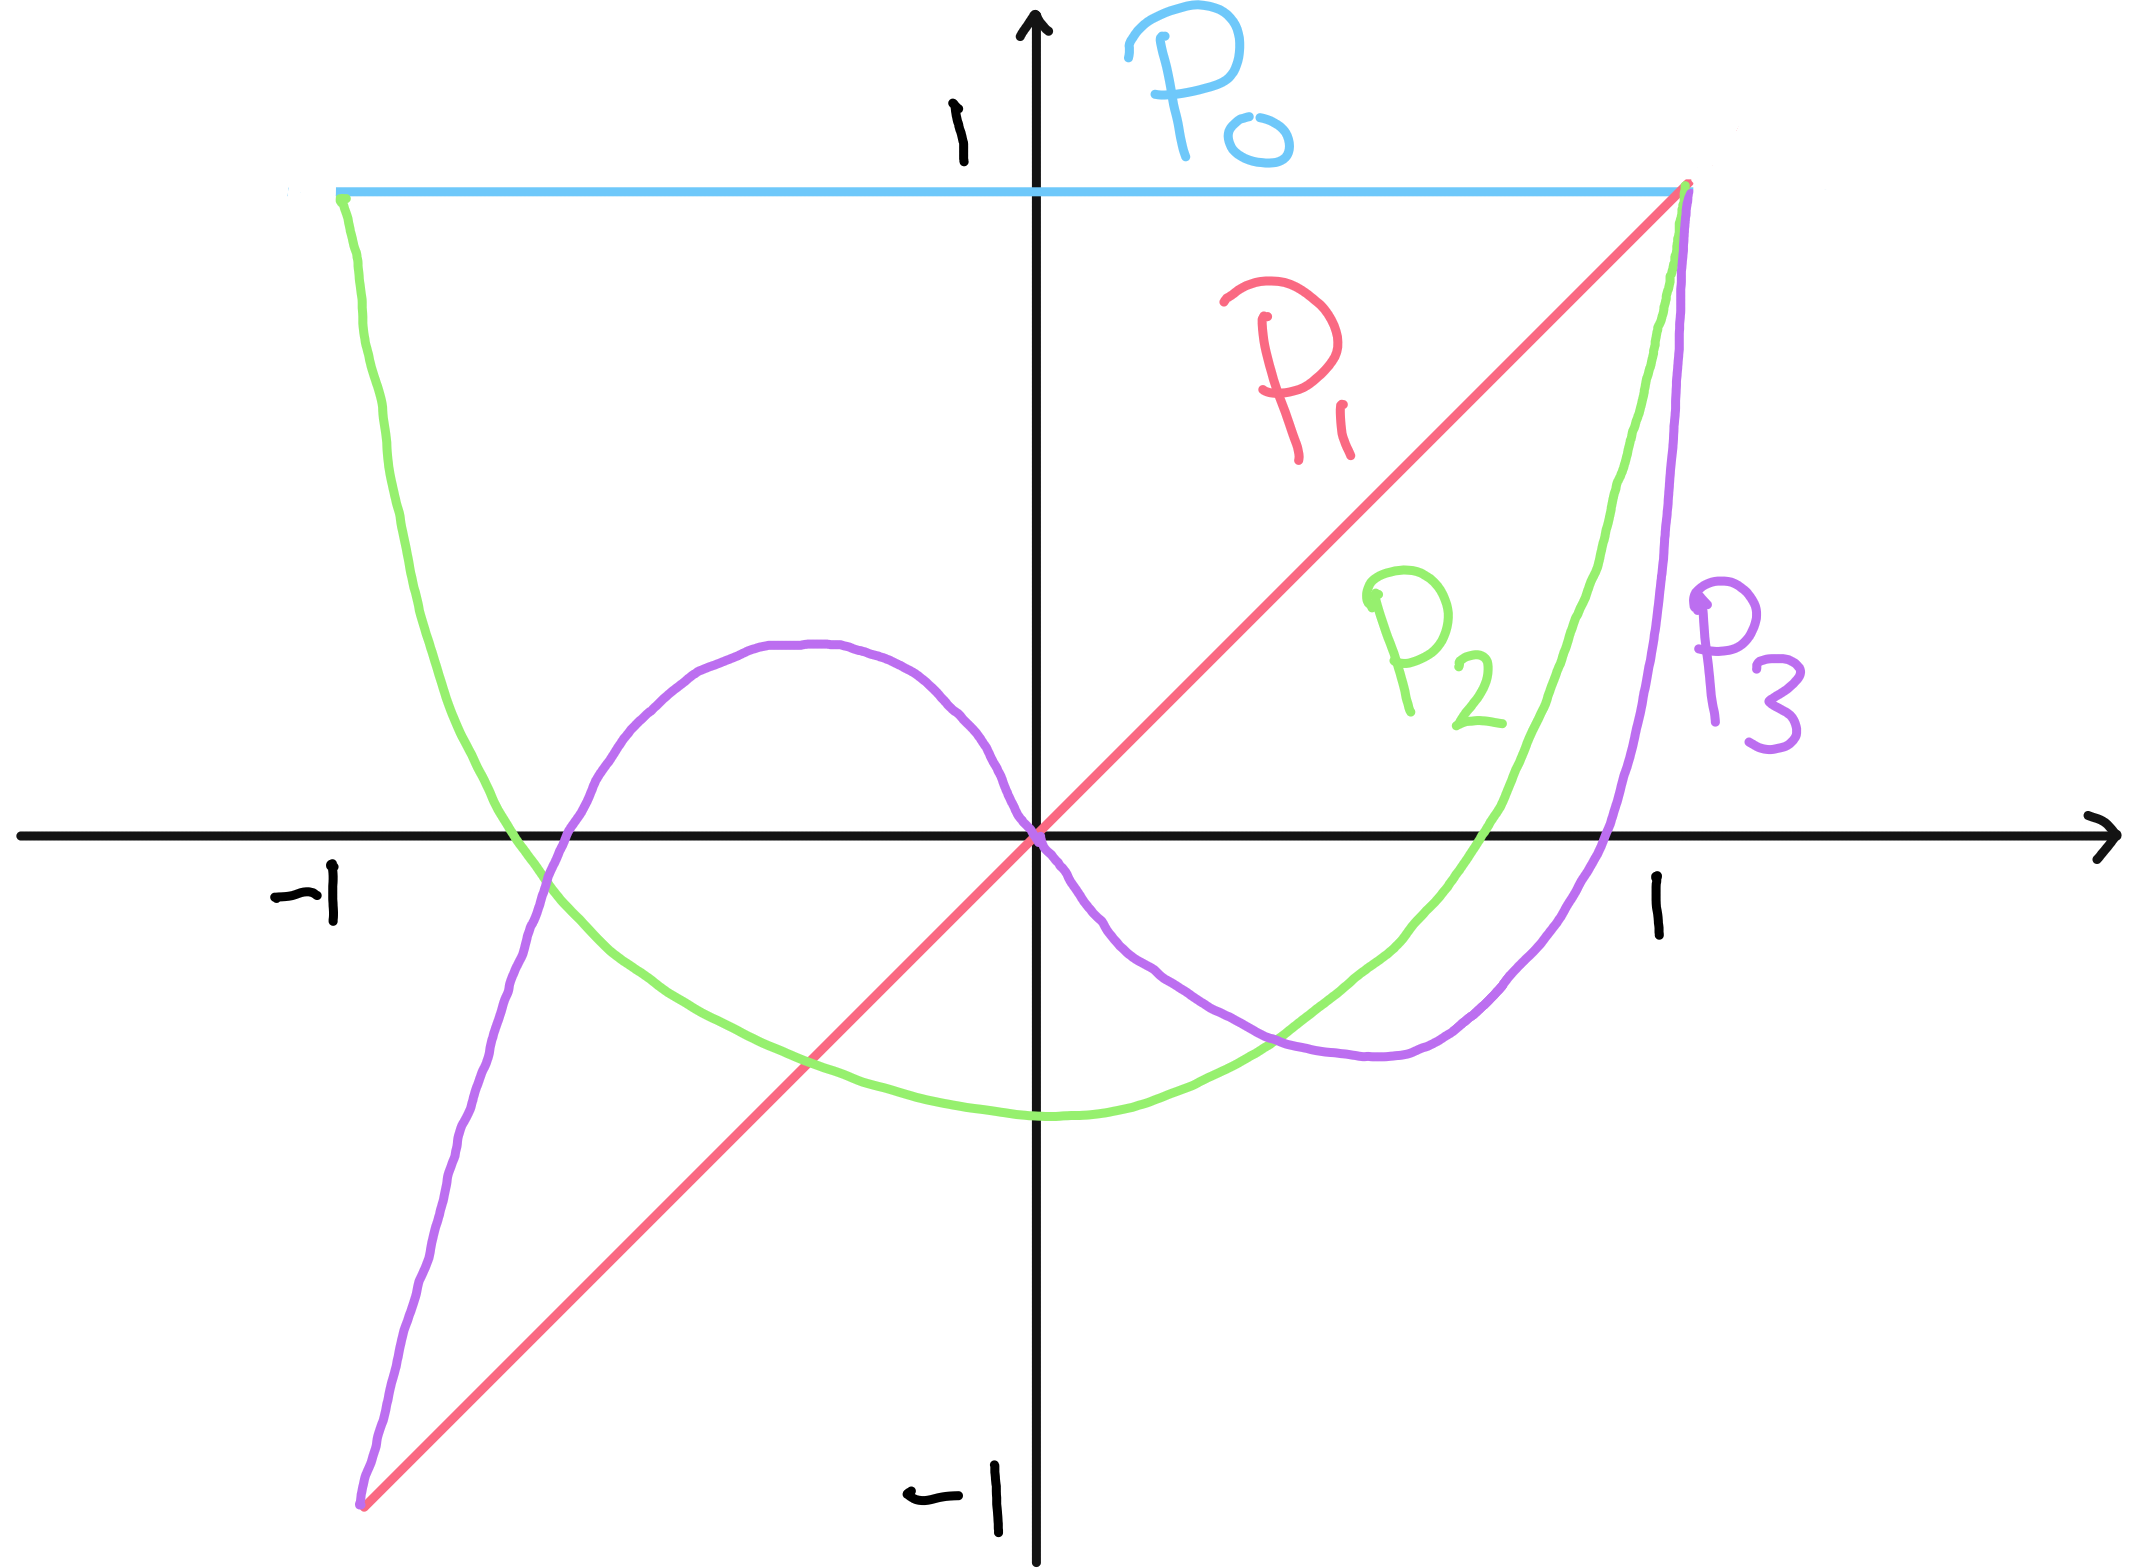
\includegraphics[height=5cm]{02-legendre} 
\end{figure}
\begin{note}
    $P_\ell(x)$ has $\ell$ zeroes.
    $P_\ell$ is odd if $\ell$ is odd, $P_\ell$ is even for even $\ell$.
\end{note} 

\subsection{Properties of Legendre polynomials}
Since Legendre polynomials come from a self-adjoint operator, they must have certain conditions, such as orthogonality.
For $n \neq m$,
\begin{align*}
    \int_{-1}^1 P_n P_m \dd{x} = 0
\end{align*}
They are also normalisable,
\addtocounter{equation}{1}
\begin{align} \label{eq:2.24}
    \int_{-1}^1 P_n^2 \dd{x} = \frac{2}{2n+1}
\end{align}
We can prove this with Rodrigues' formula (Sheet 2, Q5):
\begin{align*}
    P_n(x) = \frac{1}{2^n n!} \qty( \dv{x} )^n (x^2 - 1)^n
\end{align*}
Alternatively we could use a generating function:
\addtocounter{equation}{-2}
\begin{subequations}
    \begin{align} \label{eq:2.23a}
        \sum_{n=0}^\infty P_n(x) t^n &= \frac{1}{\sqrt{1 - 2xt + t^2}} \\
        &= 1 + \frac{1}{2}\qty(2xt - t^2) + \frac{3}{8}\qty(2xt - t^2)^2 + \dots \notag \\
        & = 1 + xt + \frac{1}{2}\qty(3x^2 - 1)t^2 + \dots \notag \\
        &= P_0 + P_1 t + P_2 t^2 + \dots \notag
    \end{align}
\end{subequations}

\begin{exercise}
    Verify $P_3$ and find $P_4$ using binomial expansion.
\end{exercise} 
There are some useful recursion relations\footnote{Derived in Example Sheet}.
\begin{align*}
    \ell(\ell + 1) P_{\ell + 1}(x) = (2 \ell + 1) x P_\ell(x) - \ell P_{\ell - 1}(x)
\end{align*}
Also,
\begin{align*}
    (2\ell + 1)P_\ell(x) = \dv{x} \qty[ P_{\ell + 1}(x) - P_{\ell - 1}(x) ]
\end{align*}

\subsection{Legendre polynomials as eigenfunctions}
Any (well-behaved) function $f(x)$ on $[-1,1]$ can be expressed as
\addtocounter{equation}{1}
\begin{align} \label{eq:2.25}
    f(x) = \sum_{\ell = 0}^\infty a_\ell P_\ell(x)
\end{align}
where
\begin{align} \label{eq:2.26}
    a_\ell = \frac{2\ell + 1}{2} \int_{-1}^1 f(x) P_\ell(x) \dd{x}
\end{align}
with no boundary conditions (e.g.\ periodicity conditions) on $f$.

\begin{exercise}
    Verify $f(x) = \frac{15}{2} x^2 - \frac{3}{2} = P_0(x) + 5 P_2(x)$ using \cref{eq:2.26}
\end{exercise} 

\subsection{Solving inhomogeneous differential equations}
\textit{This can be thought of as the general case of Fourier series discussed previously.}

Consider the problem
\begin{align} \label{eq:2.27}
    \mathcal L y = f(x) \equiv w(x) F(x)
\end{align}
on $x \in [a,b]$ assuming homogeneous boundary conditions.
Given eigenfunctions $y_n(x)$ satisfying $\mathcal L y_n = \lambda_n w y_n$, we wish to expand this solution as (recall \cref{sec:1.6})
\begin{align*}
    y(x) = \sum_n c_n y_n(x)
\end{align*}
and
\begin{align*}
    F(x) = \sum_n a_n y_n(x)
\end{align*}
where $a_n$ are known and $c_n$ are unknown.
Using \cref{eq:2.17}:
\begin{align*}
    a_n = \frac{\int_a^b w F y_n \dd{x}}{\int_a^b w y_n^2 \dd{x}}
\end{align*}
Substituting,
\begin{align*}
    \mathcal L y = \mathcal L \sum_n c_n y_n = w \sum_n c_n \lambda_n y_n = w \sum_n a_n y_n
\end{align*}
By orthogonality,
\begin{align*}
    c_n \lambda_n = a_n \implies c_n = \frac{a_n}{\lambda_n}
\end{align*}
In particular,
\begin{align} \label{eq:2.28}
    y(x) = \sum_{n=1}^\infty \frac{a_n}{\lambda_n}y_n(x)
\end{align} (assuming $\lambda_n \neq 0, \forall \; n$).

We can further generalise; we can permit a driving force, which often induces a linear response term $\widetilde\lambda w y$.
\begin{align} \label{eq:2.29}
    \mathcal L y - \widetilde \lambda w y = f(x)
\end{align}
where $\widetilde \lambda$ is fixed.
The solution \cref{eq:2.28} becomes
\begin{align} \label{eq:2.30}
    y(x) = \sum_{n=1}^\infty \frac{a_n}{\lambda_n - \widetilde \lambda} y_n(x)
\end{align} (again $\widetilde \lambda \neq \lambda_n, \forall \; n$).

\subsection{Integral solutions and Green's function}
Recall \cref{eq:2.28}
\begin{align*}
    y(x) = \sum_{n=1}^\infty \frac{a_n}{\lambda_n} y_n(x) = \sum_n \frac{y_n(x)}{\lambda_n N_n} \int_a^b w(\xi) F(\xi) y_n(\xi) \dd{\xi} \text{ by \cref{eq:2.17}}
\end{align*}
where
\begin{align*}
    N_n = \int w y_n^2 \dd{x}
\end{align*}
This then gives
\begin{align}
    y(x) &= \int_a^b \underbrace{\sum_{n=1}^\infty \frac{y_n(x) y_n(\xi)}{\lambda_n N_n}}_{G(x,\xi)} \underbrace{w(\xi) F(\xi)}_{f(\xi)} \dd{\xi} \notag\\
    &= \int_a^b G(x;\xi) f(\xi) \dd{\xi} \label{eq:2.31}
\end{align}
where
\begin{align*}
    G(x,\xi) = \sum_{n=1}^\infty \frac{y_n(x) y_n(\xi)}{\lambda_n N_n}
\end{align*}
is the eigenfunction expansion of the Green's function.
Note that the Green's function does not depend on $f$, but only on $\mathcal L$ and the boundary conditions.
In this sense, it acts like an inverse operator
\begin{align*}
    \mathcal L\inv \equiv \int \dd{\xi} G(x,\xi)
\end{align*}
analogously to how $Ax = b \implies x = A^{-1} b$ for matrix equations.